\documentclass[12pt,twoside]{report}
\usepackage{hyperref}
\usepackage{graphicx}
\usepackage{amsmath, amssymb}
\usepackage[table]{xcolor}
\usepackage{amssymb}
\usepackage{csquotes}

\newtheorem{theorem}{Theorem}
% Ctrl + Alt + B

%%%%%%%%%%%%%%%%%%%%%%%%%%%%%%%%%%%%%%%%%%%%%%%%%%%%%%%%%%%%%%%%%%%%%%%%%%%%%

% Definitions for the title page
% Edit these to provide the correct information
% e.g. \newcommand{\reportauthor}{Timothy Kimber}
\DeclareMathOperator{\E}{\mathbb{E}}

\newcommand{\reporttitle}{Symbolic Reinforcement Learning using Inductive Logic Programming}
\newcommand{\reportauthor}{Kiyohito Kunii}
\newcommand{\supervisor}{Professor Alessandra Russo}
\newcommand{\degreetype}{MSc in Computing Science}

%%%%%%%%%%%%%%%%%%%%%%%%%%%%%%%%%%%%%%%%%%%%%%%%%%%%%%%%%%%%%%%%%%%%%%%%%%%%%

% load some definitions and default packages
%%%%%%%%%%%%%%%%%%%%%%%%%%%%%%%%%%%%%%%%%
% University Assignment Title Page
% LaTeX Template
% Version 1.0 (27/12/12)
%
% This template has been downloaded from:
% http://www.LaTeXTemplates.com
%
% Original author:
% WikiBooks (http://en.wikibooks.org/wiki/LaTeX/Title_Creation)
%
% License:
% CC BY-NC-SA 3.0 (http://creativecommons.org/licenses/by-nc-sa/3.0/)
%
%
%%%%%%%%%%%%%%%%%%%%%%%%%%%%%%%%%%%%%%%%%
%----------------------------------------------------------------------------------------
%	PACKAGES AND OTHER DOCUMENT CONFIGURATIONS
%----------------------------------------------------------------------------------------
\usepackage[a4paper,hmargin=2.8cm,vmargin=2.0cm,includeheadfoot]{geometry}
\usepackage{textpos}
\usepackage[numbers]{natbib} % for bibliography
\usepackage{tabularx,longtable,multirow,subfigure,caption}%hangcaption
\usepackage{fncylab} %formatting of labels
\usepackage{fancyhdr} % page layout
\usepackage{url} % URLs
\usepackage[english]{babel}
\usepackage{amsmath}
\usepackage{graphicx}
\usepackage{dsfont}
\usepackage{epstopdf} % automatically replace .eps with .pdf in graphics
\usepackage{backref} % needed for citations
\usepackage{array}
\usepackage{latexsym}

% \usepackage[pdftex,pagebackref,hypertexnames=false,colorlinks]{hyperref} % provide links in pdf
\usepackage{hyperref}
\hypersetup{pdftitle={},
  pdfsubject={},
  pdfauthor={},
  pdfkeywords={},
  pdfstartview=FitH,
  pdfpagemode={UseOutlines},% None, FullScreen, UseOutlines
  bookmarksnumbered=true, bookmarksopen=true, colorlinks,
    citecolor=black,%
    filecolor=black,%
    linkcolor=black,%
    urlcolor=black}

\usepackage[all]{hypcap}


%\usepackage{color}
%\usepackage[tight,ugly]{units}
%\usepackage{float}
%\usepackage{tcolorbox}
%\usepackage[colorinlistoftodos]{todonotes}
% \usepackage{ntheorem}
% \theoremstyle{break}
% \newtheorem{lemma}{Lemma}
% \newtheorem{theorem}{Theorem}
% \newtheorem{remark}{Remark}
% \newtheorem{definition}{Definition}
% \newtheorem{proof}{Proof}


%%% Default fonts
\renewcommand*{\rmdefault}{bch}
\renewcommand*{\ttdefault}{cmtt}



%%% Default settings (page layout)
\setlength{\parindent}{0em}  % indentation of paragraph

\setlength{\headheight}{14.5pt}
\pagestyle{fancy}
\renewcommand{\chaptermark}[1]{\markboth{\chaptername\ \thechapter.\ #1}{}}

\fancyfoot[ER,OL]{\sffamily\textbf{\thepage}}%Page no. in the left on odd pages and on right on even pages
\fancyfoot[OC,EC]{\sffamily }
\renewcommand{\headrulewidth}{0.1pt}
\renewcommand{\footrulewidth}{0.1pt}
\captionsetup{margin=10pt,font=small,labelfont=bf}


%--- chapter heading

\def\@makechapterhead#1{%
  \vspace*{10\p@}%
  {\parindent \z@ \raggedright \sffamily
    \interlinepenalty\@M
    \Huge\bfseries \thechapter \space\space #1\par\nobreak
    \vskip 30\p@
  }}

%---chapter heading for \chapter*
\def\@makeschapterhead#1{%
  \vspace*{10\p@}%
  {\parindent \z@ \raggedright
    \sffamily
    \interlinepenalty\@M
    \Huge \bfseries  #1\par\nobreak
    \vskip 30\p@
  }}

\allowdisplaybreaks


% load some macros
% Here, you can define your own macros. Some examples are given below.

\newcommand{\R}[0]{\mathds{R}} % real numbers
\newcommand{\Z}[0]{\mathds{Z}} % integers
\newcommand{\N}[0]{\mathds{N}} % natural numbers
\newcommand{\C}[0]{\mathds{C}} % complex numbers
\renewcommand{\vec}[1]{{\boldsymbol{{#1}}}} % vector
\newcommand{\mat}[1]{{\boldsymbol{{#1}}}} % matrix


\date{June 2018}

\begin{document}
% \theoremstyle{definition}
\newtheorem{examp}{Example}[section]
% load title page
% Last modification: 2015-08-17 (Marc Deisenroth)
\begin{titlepage}

\newcommand{\HRule}{\rule{\linewidth}{0.5mm}} % Defines a new command for the horizontal lines, change thickness here


%----------------------------------------------------------------------------------------
%	LOGO SECTION
%----------------------------------------------------------------------------------------


\includegraphics[width = 4cm]{./figures/imperial}\\[0.5cm] 

\center % Center remainder of the page

%----------------------------------------------------------------------------------------
%	HEADING SECTIONS
%----------------------------------------------------------------------------------------

\textsc{\Large Imperial College London}\\[0.5cm] 
\textsc{\large Department of Computing}\\[0.5cm] 

%----------------------------------------------------------------------------------------
%	TITLE SECTION
%----------------------------------------------------------------------------------------

\HRule \\[0.4cm]
{ \huge \bfseries \reporttitle}\\ % Title of your document
\HRule \\[1.5cm]
 
%----------------------------------------------------------------------------------------
%	AUTHOR SECTION
%----------------------------------------------------------------------------------------

\begin{minipage}{0.4\textwidth}
\begin{flushleft} \large
\emph{Author:}\\
\reportauthor % Your name
\end{flushleft}
\end{minipage}
~
\begin{minipage}{0.4\textwidth}
\begin{flushright} \large
\emph{Supervisor:} \\
\supervisor % Supervisor's Name
\end{flushright}
\end{minipage}\\[4cm]


%----------------------------------------------------------------------------------------
%	FOOTER & DATE SECTION
%----------------------------------------------------------------------------------------
\vfill % Fill the rest of the page with whitespace
Submitted in partial fulfillment of the requirements for the MSc degree in
\degreetype~of Imperial College London\\[0.5cm]

\makeatletter
\@date 
\makeatother


\end{titlepage}


% page numbering etc.
\pagenumbering{roman}
\clearpage{\pagestyle{empty}\cleardoublepage}
\setcounter{page}{1}
\pagestyle{fancy}

%%%%%%%%%%%%%%%%%%%%%%%%%%%%%%%%%%%%
% \begin{abstract}
% Your abstract.
% \end{abstract}
%
% \cleardoublepage
%%%%%%%%%%%%%%%%%%%%%%%%%%%%%%%%%%%%
% \section*{Acknowledgments}
% Comment this out if not needed.
%
% \clearpage{\pagestyle{empty}\cleardoublepag e}

%%%%%%%%%%%%%%%%%%%%%%%%%%%%%%%%%%%%
%--- table of contents
\fancyhead[RE,LO]{\sffamily {Table of Contents}}
\tableofcontents

% ADD BLANK PAGE
% \clearpage{\pagestyle{empty}\cleardoublepage}
\pagenumbering{arabic}
\setcounter{page}{1}
\fancyhead[LE,RO]{\slshape \rightmark}
\fancyhead[LO,RE]{\slshape \leftmark}

%%%%%%%%%%%%%%%%%%%%%%%%%%%%%%%%%%%%
\chapter{Introduction}
% IMPERIAL LOGO
% \begin{figure}[tb]
% \centering
% 
\includegraphics[width = 0.4\hsize]{./figures/imperial}
% \caption{Imperial College Logo. It's nice blue, and the font is quite stylish. But you can choose a different one if you don't like it.}
% \label{fig:logo}
% \end{figure}
% Figure~\ref{fig:logo} is an example of a figure.


There has been successful applications of deep reinforcement learning (DRL) a number of domains, such as games and robotics (TODO INSERT REFERENCES).
DRL is considered to be a step towards artificial general intelligence.
As pointed by XXX, however, there are still a number of issues to overcome in this method.
First, it requires a large amount of data for training the model, which requires a long time of learning process.
Second, it is considered to be a black-box, meaning the decision making process is unknown to human user and therefore lacks explanation ability.
Third there is no thoughts process to the decision making, which, as XX points out, is a fundamental to the artificial general intelligence.
To tackle these problems, there are 3 main streams of research on this field.
First main research is focused on applying Baysian statistics XXX, the second main research is XXX.
Recently, the XXX attempted to incorporate symbolic representations into the system to achive more data-efficient learning, which shows a promissing results of this approach.

MOTIVATION

Why symbolic reinforcement learning is good attempt


Reason 1: Complehensive by humans $\rightarrow$ Explanable rather than black-box

Reason 2: Similar to the human, it uses reasoning

Use of previous experience (background knowledge)
As discussed in XX, there are many research that attempted to incorporate symbolic reasoning into DRL, but there is not much research on incorporating symbolc learning with reinforcement learning

However there is a room for exploration on this field.

Reason 3: Recent advance of ILASP is promissing

Because of the recent advancement of logic-based learning and deep reinforcement learning, combination of both approach would be a next explonation toward artificial general intelligence.


OBJECTIVES
combining the two novel approaches to overcome the problems of the QND





In this paper, I further explore incorporation of symbolic machine learning into reinforcement learning to achieve data-efficient learning using Inductive Learning of Answer Set Programs (ILASP), which is the state-of-art symbolic learning method that can be applied to imcomplete and more complex environment.
This research is inspired by \cite{Garnelo2016}, but in this paper I explore symbolic represetations process and include more learning aspect.

This background report is organised as follows: Chapter \ref{background} introduces

\chapter{Background}
\label{background}

This section introduces introduces Inductive Logic Programming (Section \ref{ilp}), Reinforcement Learning (Section \ref{rl}) and GVGAI Framework, an open-source game platform for AI methods (Section \ref{gvgai}), which provide the foundations of this work.

\section{Logic Basics}

TODO ENTAILMENT

To compute this inference task, the syntax of the predicate logic program needs to be converted into Conjunctive Normal Form (CNF), or clausal theory, which consists of a conjunction of clauses, where a clause is disjunction of literals, and a literal can include positive literals and negative literals.

A literal is either an atom p or negation by failure, which is used to derive not p.

\begin{examp} (Conjunctive Normal Form)

\end{examp}


The \textit{Herbrand domain} (a.k.a \textit{Herbrand universe}) of clause sets \textit{Th} is the set of all ground terms that are constants and function symbols appeared in \textit{Th}.

\begin{examp} (Herbrand Domain)

\end{examp}

The \textit{Herbrand base} of \textit{Th} is the set of all ground predicates that are formed by predicate symbols in \textit{Th} and terms in the \textit{Herbrand domain}.

\begin{examp} (Herbrand Base)

\end{examp}

The \textit{grounding} of \textit{Th} is the set of all clauses that are c $\in$ \textit{Th} and variables are replaced by terms in the \textit{Herbrand Domain}.

\begin{examp} (Grounding)

\end{examp}


TODO Explain grounding in ASP context.


A \textit{Horn clause} is a subset of CNF, which is a clause wtith at most one positive literal, where a \textit{definite clause} (also called a \textit{rule} or a \textit{fact}) contains exactly one positive literal, and a \textit{denial} (or a \textit{constraint}) is a clause with no positive literals.

\begin{examp} (Horn clause)

\end{examp}



Limitations of Inductive Logic Programming:

\subsection{Stable Model Semantics}

TODO Relationship from the previous Section

Definite Logic Program is a set of definite rule where: \newline

a definite rule is of the form h $\leftarrow$ a\textsubscript{1}, ..., a\textsubscript{n}, where h , a\textsubscript{1}, ..., a\textsubscript{n} are all atoms.

whereas

Normal Logic Program is a set of normal rule where

a normal rule is of the form h $\leftarrow$ a\textsubscript{1}, ..., a\textsubscript{n}, \textit{not} b\textsubscript{1}, ..., \textit{not}  b\textsubscript{n} where h is the head of the rule,
 and a\textsubscript{1}, ..., a\textsubscript{n}, b\textsubscript{1}, ..., b\textsubscript{n} are the body of the rule (both the head and body are all atoms).


The grounding of a normal logic program P can be obtained by replacing each rule in P with a ground instance of the rule, such that for each atom A in body\textsuperscript{+} (R) (TODO EXPLAIN WHAT THIS IS), already occurs in the head of another ground rule.


RELATIONSHIP WITH PROLOG

The entire program needs to be grounded in order for ASP solver to work, and, unlike Prolog,  each rule must be \enquote{safe}. A rule R is safe if every variable that occurs in the head of the rule occurs at least once in body\textsuperscript{+}(R) (TODO check if this is correct).

An \textit{Herbrand interpretation} of a set of definite clauses \textit{Th} is a subset of the Herbrand base of \textit{Th}, which is a set of ground atoms that are true in terms of interpretation.



Interpretation evaluate it to true
Interpretation evaluate it to false

A \textit{Herbrand Model} is a Herbrand interpretation if and only if a set Th of clauses is satisfiable.


Algorithm for computing Herbrand model is shown in

XXXX

A set of clauses Th is unsatisfiable if the algorithm terminates and does not return Herbrand model.

The \textit{Least Herbrand Model} is an unique minimum Herbrand model if and only if none of its subsets is an Herbrand model (TODO MATHMATICALLY SAY THIS)

For a normal program, there is usually no least Herbrand model.
TODO Explain MORE

Stable Model of a normal logic program is XX
\cite{Gelfond1988}

Any stable model is a minimal Herbrand model, and stable sets is stable models. The stable models can be found by constructing the result of the program with respect to sets of atoms X (P\textsuperscript{x} in the following 2 steps



does not contain negation and a unique minimal Herbrand model.

\begin{examp} (Horn clause)

\end{examp}


\subsection{Anwer Set Programming (ASP)}

Answer set of normal logic program P is a stable model, and Answer Set Programming (ASP) is a normal logic program with extensions: constrains, choice rules and optimisation. ASP program consists of a set of rules, where each rule consists of an atom and literals.
A literal is either an atom \textit{p} or its \textit{default negation} not p (Negation as a failure).


Head and body

A Constraint is of the form

\begin{theorem}
$\leftarrow$ a\textsubscript{1}, ..., a\textsubscript{n}, not b\textsubscript{1}, ..., not b\textsubscript{n}
\end{theorem}

which is to filtering any irrelevant answer sets.
There are two types of constraints: soft and hard constraints. Soft constraint is XXX

Hard constraint is XXX

Choice rule can express possible outcomes given an action choice, which is of the form

\begin{theorem}
l{h\textsubscript{1},...,h\textsubscript{m}}u $\leftarrow$ a\textsubscript{1}, ..., a\textsubscript{n}, not b\textsubscript{1}, ..., not b\textsubscript{n}
\end{theorem}

where the head is called \textit{aggregates}.

An answer set of ASP program is interpretations that make all the ruls true.

Non-monotonicity.

ASP has true, false and unknown

for non-deterministic to describe transition possibilities.

% DO I NEED OPTIMISATION??
optimisation statement is of the form.

Which is useful to order the answer sets in terms of preference.

\textit{Clingo} is one of the programs to execute the ASP program and returns answer sets of the programs.

\section{Inductive Logic Programming (ILP)}

\label{ilp}
Inductive Logic Programming (ILP) is a subfield of research area aimed at the intersection between machine learning and logic programming \cite{Muggleton1991}. The purpose of ILP is to inductively derive a hypothesis H that is a solution of a learning task, which coveres all positive examples and any of negative examples.

ENTAILMENT

Satisfiable

\begin{equation}
B \cap H \models E
\end{equation}

where E consists of positive examples (E\textsuperscript{+}) and negative examples (E\textsuperscript{-})


\subsubsection{ILP in Anser set semantics}

Cautious and brave entailments can be defined in terms of induction in ILP \cite{Sakama2009}.

% Sakama 2008 has no concept of negative examples in this paper.

Cautious Induction task is of the form $\langle$ B, E\textsuperscript{+}, E\textsuperscript{-} $\rangle$ where: \\
B is the background knowledge \\
E\textsuperscript{+} is a set of positive examples \\
E\textsuperscript{-} is a set of negative examples \\

 H $\in$ ILP\textsubscript{cautious} $\langle$ B, E\textsuperscript{+}, E\textsuperscript{-} $\rangle$ if and only if  \\

 there is at least one answer set A of B $\cup$ H such that: \\
 for every anser set A of B $\cup$ H:
$\forall$ e $\in$ E\textsuperscript{+} : e $\in$ A \\
$\forall$ e $\in$ E\textsuperscript{-} : e $\notin$ A \\

\begin{examp} (Limitation of cautious induction)

1\{situation(P, awake), situation(P, sleep)\}1 :- person(P).

person(john).
\end{examp}
\label{limitation_cautious}

In the example \ref{limitation_cautious}, neither of situation(john, awake) or situation(john, sleep) is false in all answer sets. In this example, it only return person(john).

Cautious entailment may be too restrict.

Similarly, Brave Induction task is of the form $\langle$ B, E\textsuperscript{+}, E\textsuperscript{-} $\rangle$ where: \\
B is the background knowledge \\
E\textsuperscript{+} is a set of positive examples \\
E\textsuperscript{-} is a set of negative examples \\

 H $\in$ ILP\textsubscript{brave} $\langle$ B, E\textsuperscript{+}, E\textsuperscript{-} $\rangle$ if and only if there is at least one answer set A of B $\cup$ H such that: \\
$\forall$ e $\in$ E\textsuperscript{+} : e $\in$ A \\
$\forall$ e $\in$ E\textsuperscript{-} : e $\notin$ A \\


By contrast, Brave indction is that it cannot learn constrains as shown in the example \ref{limitation_brave}.

\begin{examp} (Limitation of brave induction)

XXX
\end{examp}
\label{limitation_brave}

\subsection{Learning from Anwer Sets (LAS)}

Cautious induction In order to overcome the limitations of cautious and brave induction,
Learning from Answer Sets (LAS) was developed in \cite{Law2014} to faciliate more complex learning task.

Examples used in LAS is converted from $\langle$ E\textsuperscript{+}, E\textsuperscript{-}$\rangle$ into

Partial Interpretations are of the form $\langle$ E\textsuperscript{inc}, E\textsuperscript{exc}$\rangle$

A Herbrand Interpretations extends a partial interpretation if it include all of the inclusions and none of the exclusions.

\subsection{Inductive Learning of Answer Set Programs (ILASP)}

ILASP is an algorithm that is capable of solving LAS tasks

It is based on two fundamental concepts: positive solutions and violating solutions.
A hypothesis H is a positive solution if and only if
1. H $\subseteq$ S\textsubscript{M} \\
2. $\forall$ e\textsuperscript{+} $\in$ $\exists$ A $\in$ AS(B $\cup$ H) subject to A extends e\textsuperscript{+}\\

A hypothesis H is a violating solution if and only if
1. H $\subseteq$ S\textsubscript{M} \\
2. $\forall$ e\textsuperscript{+} $\in$ E\textsuperscript{+} $\exists$ A $\in$ AS(B $\cup$ H) subject to A extends e\textsuperscript{+}\\
3. $\exists$ e\textsuperscript{-} $\in$ E\textsuperscript{-} $\exists$ A $\in$ AS(B $\cup$ H) subject to A extends e\textsuperscript{-}\\


ILP\textsubscript{LAS} is positive solutions that are not violating solutions.

ILASP task containing a contex-dependent example

TODO Explain how symbolic learning works

TODO What would you learn in my context? Relashinship of the objects?
Objects, types, locations and interactions.

\section{Reinforcement Learning}
\label{rl}

\begin{figure}[!htb]
\centering
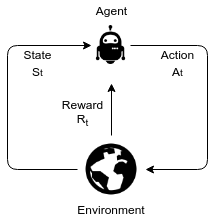
\includegraphics[width=5cm, height=5cm]{./figures/agent_env}
\caption{Agent and Environment}
\label{agent_env}
\end{figure}

% An RL agent may include either Policy, Value function or Model,

On-Policy learn policy $\pi$ from its past experience
Off-policy

Model-based vs model-free learning

\subsection{Markov Decision Process(MDP)}


(Puterman, 1994)
There is an agent who interacts with an envirnment (Figure \ref{agent_env}). At each time step, an action taken by the agent affect the environment state and the reward (or penality) it receives from the action outcome. (TODO Observations)
When an agnet must make a sequence of decision, the sequential decision problem can be formalised using Markov decision process (MDP). MDPs formaly represent a fully observable environment of an agent for reinforcement learning.

A MDP is of the form $\langle$ S, A, T\textsubscript{a}, R\textsubscript{a}, $\gamma$ $\rangle$ where: \\

\begin{itemize}
\item S is the set of finite states that is observable in the environment
\item A is the set of finite actions taken by the agent
\item T\textsubscript{a}(s, s$^\prime$) is a state transition in the form of probability matrix Pr(S\textsubscript{t+1} = s$^\prime$ $\vert$ s\textsubscript{t} = s, a\textsubscript{t} = a), which is the probablity that action a in state s at time t will result in state s$^\prime$ at time t+1.
\item R is a reward function R\textsubscript{a}(s, s$^\prime$) = $\displaystyle \E[R\textsubscript{t+1} $ $\vert$ S\textsubscript{t} = s, A\textsubscript{t} = a], the expected immediate reward that action a in state s at time t will return
\item $\gamma$ is a discount factor $\gamma$ $\in$ [0,1], which represents the preference of the agent for present rewards over future rewards

\end{itemize}

In MDPs, there is an element of delayed reward tradeoff between immediate rewards and its delayed reward

A state S\textsubscript{t} is Markov if and only if
P[S\textsubscript{t+1} $\vert$ S\textsubscript{t}] = P[S\textsubscript{t+1} $\vert$ S\textsubscript{1}, ..., S\textsubscript{t}] therefore the probability of reaching S\textsubscript{t+1} depends solely on S\textsubscript{t}, which captures all the relevant information from earilier history.

A solution to the sequential decision problem is called a policy $\pi$, a sequence of actions that leads to a solution
% which is a distributin over actions given states.

The transition and reward functions are not necessary to be known to compute $\pi$.

An optimal policy $\pi^*$ is the one that maximise the total rewards in the environment.

The total reward with a discount factor is



The existence of the discount factor can be justified as follows:

TODO
$\displaystyle \E[R\textsubscript{t+1} \vert$ S\textsubscript{t} = s]


Reinforcement learning is a method to get approximated optimal solution.


\subsection{Temporal-Difference (TD) Learning}

To solve MDP, one of the approaches is called Temporal-Difference (TD) Learning.

TD learns directly from episodes of experiences, which can be imcomplete.
TD does not require knowledge of MDP transitions and rewards (model-free)
Sutton 1988

Update value
\begin{equation}
V(S\textsubscript{t} \leftarrow V(S\textsubscript{t} + \alpha (R\textsubscript{t+1} + \gamma V(S\textsubscript{t+1}) - V(S\textsubscript{t}))
\end{equation}

where R\textsubscript{t+1} + $\gamma$ V(S\textsubscript{t+1}) is the estimated return (a.k.a TD target)

R\textsubscript{t+1} + $\gamma$ V(S\textsubscript{t+1}) - V(S\textsubscript{t}) is TD error.

TD updates the estimate by using the estimates of XXX (bootstrap).

The advantages of TD methods
- does not require any model of an environment.
- online learning
\subsection{Q-Learning}

model-free leaning, where the agent will not rely on the models of the environment.

Q-learning approximate the Q(a,s) from the samples of

the agent only knows about the possible states and actions but the transition state and reward probability functions are unknown.

Q function is the state-action pair

the optimal Q-function Q\textsuperscript{*}(s,a) represents XXX for the agent to selection action a given that it is in state s.

Q-learning is off-policy TD learning defined in [Watkin 1989], which is of the form:
%
% \begin{equation}
% Q(s\textsubscript{t},a\textsubscript{t}) \leftarrow Q(s\textsubscript{t},a\textsubscript{t}) + \alpha(R\textsubscript{t+1} + \gamma max (a+t) Q(s\textsubscript{t+1}, a\textsubscript{t+1}) - Q(s\textsubscript{t}, a\textsubscript{t}))
%
% \end{equation}

where $\alpha$ is the learning rate, $\gamma$ is a discount rate between 0 and 1.

this equation is used to upate action-value function

Model free learning: derectly derive an optimal policy by interacting with the environment without the model

Model free can be done using Monte Carlo Policy evaluation

One way to solve the Bellman Optimality equation is Q-leraning

U(s) = max a Q(s,a)


a function Q(S,A) which predicts the best action A in state S to maximise the total cumulative rewards.

The function is estimated by Q-learning, which repeately updates Q(s,a) using
the Bellman Equation.

TODO INSERT Q-learning ALGORITHM HERE

Epsilon greedy

\section{GVGAI Framework}
\label{gvgai}

The Video Game Definition Language (VGDL)

SpriteSet defines all the sprites available in the game.
LevelMapping defines relationships among characters, and the sprites available.
InteractionSet defines what events occur when two sprites collide
TerminationSet defines the end conditions of the game, and decides whether the player wins or not.

TODO Add game images

% Timeout and SpriteCounter

%%%%%%%%%%%%%%%%%%%%%%%%%%%%%%%%%%%
\chapter{Related Work}

% \section{Deep Reinforcement Learning and its issues}

Transparency and interpretable capability of the model is another important aspect for machine learning applications.


XXX[Programmati...] developed a programmatically interpretable reinforcement learning which finds a policy that can be represented in a human-readable programming language.


Two most studied approach for using previous learning exprience is meta-learning and transfer learning

Artificial General Intelligence

Definision of AGI

The history of data-efficient learning
What other people have done in this.

The advance of statistical machine learning methods, especially deeep reinforcement learning

AlphaGo, and AlphaGo Zero

Study of symbolic machine learning roots from
% Relational Reinforcement Learning

Baysian Optimisation

RNN approach

Symbolic Deep reinforcement learning

Some implementation: German paper

The paper was the application of symbolic representatiojns into a very simple game to demonstrate this proof of concept would actually work.
By contract, there is active reserach in symbolic machine learning, which focuses on logic=based learning rather than statistical machine learning.
For example, XX shows the agent can learn XXX from a noisy examples, with only a very few training examples.


\section{Symbolic Reinforcement Learning}
Incorporation of logic into reinforcement learning dates back to the study of relational reinforcement learning,


More recently there has been a number of attempts to incorporate ASP into reinforcement learning.

There are a number of reseached conducted in applying DNN to symbolic reasoning.
For example,

[From GamePlay to Symbolic Reasoning]


However, as XX points out, 1 pixel of the game could influence the decision making of the agent.


\chapter{Project Overview}

\section{Proposed Architecture}

\section{Project outline}

The probject outline

Implement baseline performance (DQN, Q-learning, ASPRL)

Due to the complex environment of the chosen game, I will not implemnet the original DSRL, since the feature extractions from the pixel would only work in a very simple pixel environment,

Pipeline

The basic architecture follows the similar method in XXX, but I also add symbolic learning to these extracted symbolic features using ILASP.

Apply ILASP to the ASP, which involves development of the pipeline of ILASP in Python

Finally use Q-learning that allow

which measurement would you use? (grid word, something else? GVGAL games)
Summarise different types of knowledge representations (Objects ?? relationship?)

Common sense

Lastly, I will also test the capability of transfer learning for this new method.

% \section{Contribution}
%
% To my knowledge, this is the first time that both symbolic learning method is incorporated into a reinforcement learning to facilitate learning process
%
% \section{Methods}


\chapter{Ethics Checklist}
{
\renewcommand*{\arraystretch}{1.3}
\begin{longtable}{ |p{13.2cm}|p{0.6cm}|p{0.6cm}| }
\hline
 & \bf Yes & \bf No \\
\hline

\multicolumn{3}{|l|}{\cellcolor{green!25}\bf Section 1: HUMAN EMBRYOS/FOETUSES} \\
\hline

Does your project involve Human Embryonic Stem Cells? & & \checkmark\\
\hline

Does your project involve the use of human embryos? & & \checkmark\\
\hline

Does your project involve the use of human foetal tissues / cells? & & \checkmark\\
\hline

\multicolumn{3}{|l|}{\cellcolor{green!25}\bf Section 2: HUMANS} \\
\hline

Does your project involve human participants? & & \checkmark\\
\hline

\multicolumn{3}{|l|}{\cellcolor{green!25}\bf Section 3: HUMAN CELLS / TISSUES} \\
\hline

Does your project involve human cells or tissues? (Other than from “Human Embryos/Foetuses” i.e. Section 1)? & & \checkmark\\
\hline

\multicolumn{3}{|l|}{\cellcolor{green!25}\bf Section 4: PROTECTION OF PERSONAL DATA} \\
\hline

Does your project involve personal data collection and/or processing? & & \checkmark\\
\hline

Does it involve the collection and/or processing of sensitive personal data (e.g. health, sexual lifestyle, ethnicity, political opinion, religious or philosophical conviction)? & & \checkmark\\
\hline

Does it involve processing of genetic information? & & \checkmark\\
\hline

Does it involve tracking or observation of participants? It should be noted that this issue is not limited to surveillance or localization data. It also applies to Wan data such as IP address, MACs, cookies etc. & & \checkmark\\
\hline

Does your project involve further processing of previously collected personal data (secondary use)? For example Does your project involve merging existing data sets? & & \checkmark\\
\hline

\multicolumn{3}{|l|}{\cellcolor{green!25}\bf Section 5: ANIMALS} \\
\hline

Does your project involve animals? & & \checkmark\\
\hline


\multicolumn{3}{|l|}{\cellcolor{green!25}\bf Section 6: DEVELOPING COUNTRIES} \\
\hline

Does your project involve developing countries? & & \checkmark\\
\hline

If your project involves low and/or lower-middle income countries, are any benefit-sharing actions planned? & & \checkmark\\
\hline

Could the situation in the country put the individuals taking part in the project at risk? & & \checkmark\\
\hline

\multicolumn{3}{|l|}{\cellcolor{green!25}\bf Section 7: ENVIRONMENTAL PROTECTION AND SAFETY} \\
\hline

Does your project involve the use of elements that may cause harm to the environment, animals or plants? & & \checkmark\\
\hline

Does your project deal with endangered fauna and/or flora /protected areas? & & \checkmark \\
\hline

Does your project involve the use of elements that may cause harm to humans, including project staff? & & \checkmark\\
\hline

Does your project involve other harmful materials or equipment, e.g. high-powered laser systems? & & \checkmark\\
\hline


\multicolumn{3}{|l|}{\cellcolor{green!25}\bf Section 8: DUAL USE} \\
\hline

Does your project have the potential for military applications? & & \checkmark\\
\hline

Does your project have an exclusive civilian application focus? & & \checkmark\\
\hline

Will your project use or produce goods or information that will require export licenses in accordance with legislation on dual use items? & & \checkmark\\
\hline

Does your project affect current standards in military ethics – e.g., global ban on weapons of mass destruction, issues of proportionality, discrimination of combatants and accountability in drone and autonomous robotics developments, incendiary or laser weapons? & & \checkmark\\
\hline

\multicolumn{3}{|l|}{\cellcolor{green!25}\bf Section 9: MISUSE} \\
\hline

Does your project have the potential for malevolent/criminal/terrorist abuse? & & \checkmark\\
\hline

Does your project involve information on/or the use of biological-, chemical-, nuclear/radiological-security sensitive materials and explosives, and means of their delivery? & & \checkmark\\
\hline

Does your project involve the development of technologies or the creation of information that could have severe negative impacts on human rights standards (e.g. privacy, stigmatization, discrimination), if misapplied? & \checkmark& \\
\hline

Does your project have the potential for terrorist or criminal abuse e.g. infrastructural vulnerability studies, cybersecurity related project? & & \checkmark\\
\hline

\multicolumn{3}{|l|}{\cellcolor{green!25}\bf Section 10: LEGAL ISSUES} \\
\hline

Will your project use or produce software for which there are copyright licensing implications? & \checkmark& \\
\hline

Will your project use or produce goods or information for which there are data protection, or other legal implications? & & \checkmark\\
\hline

\multicolumn{3}{|l|}{\cellcolor{green!25}\bf Section 11: OTHER ETHICS ISSUES} \\
\hline

Are there any other ethics issues that should be taken into consideration? & \checkmark& \\
\hline

\end{longtable}
}


%%%%%%%%%%%%%%%%%%%%%%%%%%%%%%%%%%%%
% \chapter{Contribution}


% %%%%%%%%%%%%%%%%%%%%%%%%%%%%%%%%%%%%
% \chapter{Experimental Results}
%
%
% %%%%%%%%%%%%%%%%%%%%%%%%%%%%%%%%%%%%
% \chapter{Conclusion}


%% bibliography
\bibliographystyle{plain}
\bibliography{references}

\end{document}
